\section*{Exercice 189 -- Modélisation}
\setcounter{exo}{0}
%E3A MP 2009

%\subsection*{Asservissement de position du palier magnétique actif}

On suppose que l’action mécanique de la pesanteur sur l’ensemble mobile est égale à
l’action mécanique de compression du ressort à vide. Cela implique que la norme de l’action
mécanique du ressort à prendre en compte est : $F_{\text{Ressort}} = r_f y(t)$.

Le modèle retenu est donc le suivant (la verticale descendante est suivant $\vect{y_0}$).


\begin{center}
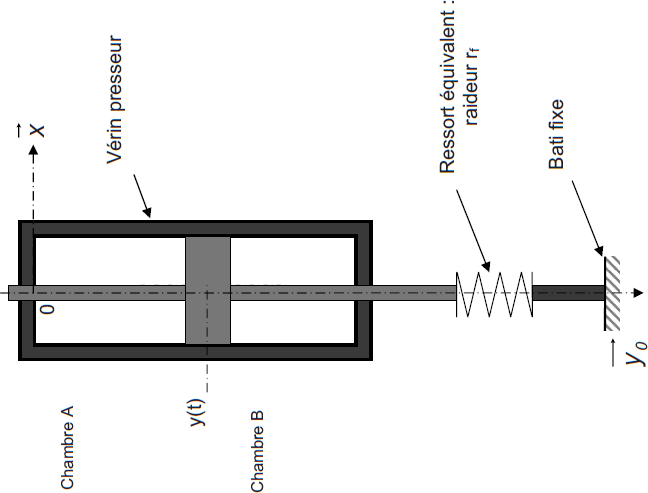
\includegraphics[width=\linewidth]{989_01}%
\end{center}

On note $M$ la masse l’ensemble mobile en translation et $y(t)$ la position du piston de la tige du vérin selon l’axe $\vect{y_0}$.




\subparagraph{}
 \textit{À partir de la figure précédente et par la méthode de votre choix, déterminer
l'équation différentielle liant $y(t)$ et ses dérivées par rapport au temps, $M$, $v$, $r_f$, $S$ et $\Delta p(t)$.}
\ifprof
\begin{corrige}
\end{corrige}
\else
\fi

\subparagraph{}
\textit{En supposant les conditions initiales nulles, exprimer dans le domaine de Laplace
l’équation établie à la question précédente. En déduire la fonction de transfert $H(p) = \dfrac{Y(p)}{P(p)}$.}
\ifprof
\begin{corrige}
\end{corrige}
\else
\fi

\subparagraph{}
 \textit{À partir de la fonction de transfert $H(p)$ et de l’équation établie précédemment, compléter le schéma-blocs suivant.}
\ifprof
\begin{corrige}
\end{corrige}
\else
\fi


\begin{center}
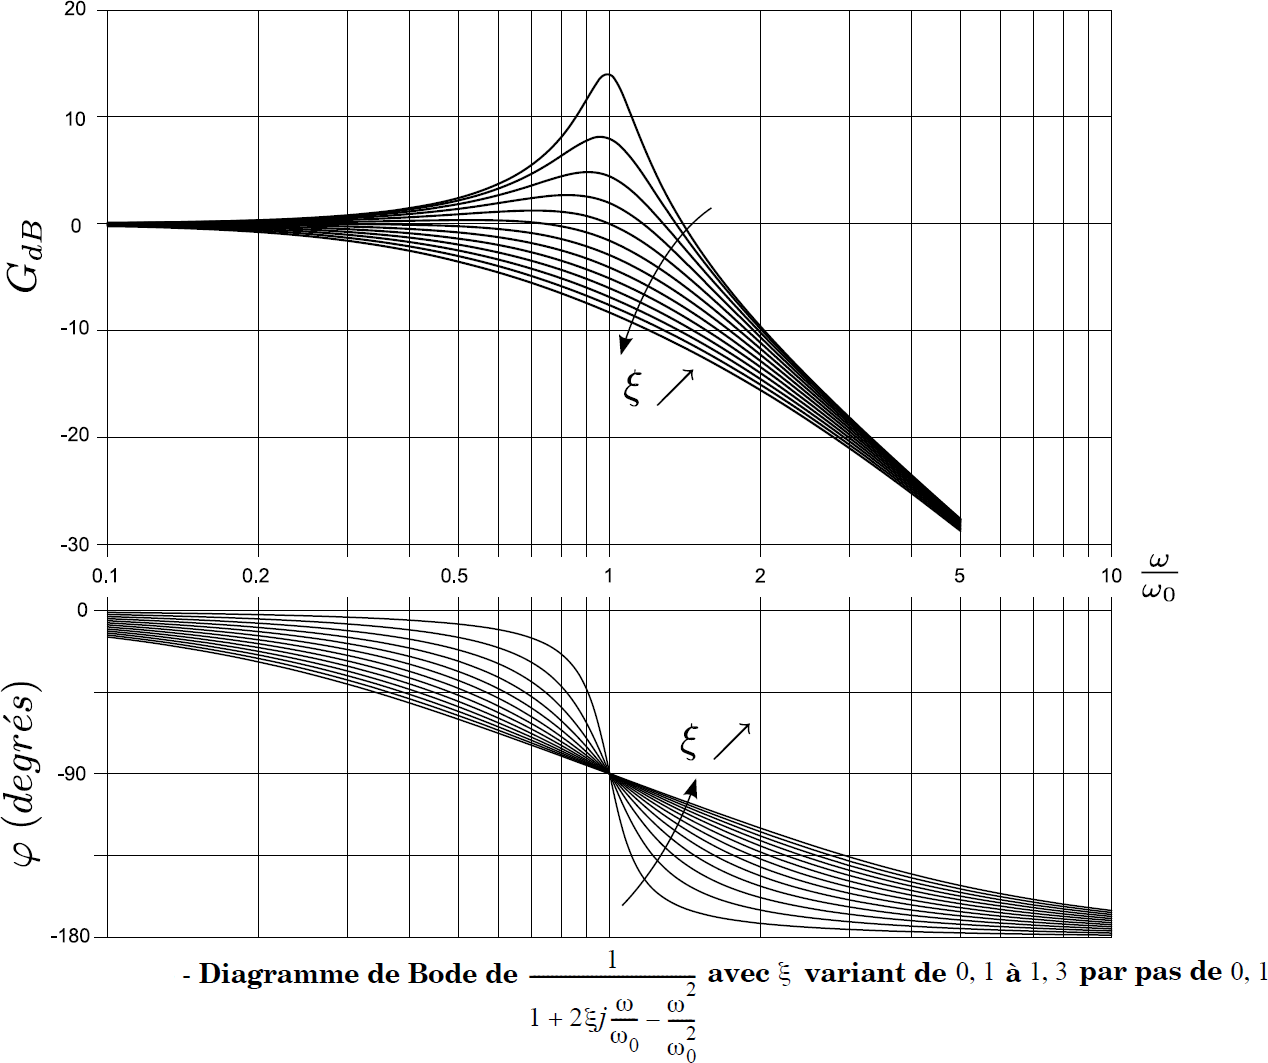
\includegraphics[width=\linewidth]{989_02}%
\end{center}

\subparagraph{}
 \textit{Donner l’expression de la fonction de transfert en boucle ouverte du système.}
\ifprof
\begin{corrige}
\end{corrige}
\else
\fi


\begin{enumerate}
\item $-v \dfrac{\dd y(t)}{\dd t} - r_f y(t) + S\Delta p(t) = M \dfrac{\dd^2 y(t)}{\dd t^2}$.
\item $H(p)=\dfrac{\dfrac{S}{r_f}}{1+\dfrac{v}{r_f}  p +  \dfrac{M}{r_f}  p^2 }$.
\item ...
\item $H_{\text{BO}}(p) = \dfrac{K_S}{1+T_S p}C(p) K_{\text{capt}} \dfrac{\dfrac{2B}{Vp}\left( 1+\dfrac{v}{r_f}  p +  \dfrac{M}{r_f}  p^2\right)}{1+\dfrac{2BS^2}{V r_f} + \dfrac{v}{r_f}  p +  \dfrac{M}{r_f}  p^2}$
\end{enumerate}